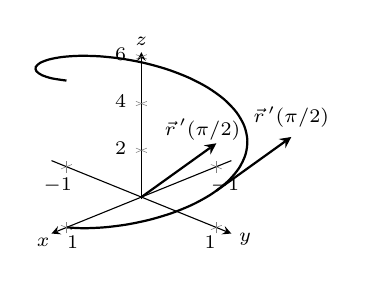
\begin{tikzpicture}[>=stealth]
\begin{axis}%
[width=175pt,tick label style={font=\scriptsize},axis on top,
			axis lines=center,
			view={135}{35},
			name=myplot,
			%xtick={-3,3},minor tick num=2,
			%ytick={-3,3},
			%ztick={-3,3},
			ymin=-1.2,ymax=1.2,
			xmin=-1.2,xmax=1.2,
			zmin=-.1, zmax=6.2,
			every axis x label/.style={at={(axis cs:\pgfkeysvalueof{/pgfplots/xmax},0,0)},xshift=-3pt,yshift=-3pt},
				xlabel={\scriptsize $x$},
			every axis y label/.style={at={(axis cs:0,\pgfkeysvalueof{/pgfplots/ymax},0)},xshift=5pt,yshift=-2pt},
				ylabel={\scriptsize $y$},
				every axis z label/.style={at={(axis cs:0,0,\pgfkeysvalueof{/pgfplots/zmax})},xshift=0pt,yshift=4pt},
				zlabel={\scriptsize $z$}
			]

\addplot3[domain=0:360,,thick,smooth,samples y=0,{\colorone},samples=30,] ({cos(x)},{sin(x)},{x/180*3.14159});

\draw[thick,->,{\colortwo}] (axis cs: 0,1,1.57) -- (axis cs: -1,1,2.57) node (A) {};
\draw[thick,->,{\colortwo}] (axis cs: 0,0,0) -- (axis cs: -1,0,1) node (B) {};


\end{axis}

\draw (A) node [ above] {\scriptsize $\vec r\,'(\pi/2)$};
\draw (B) node [shift={(-5pt,5pt)}] {\scriptsize $\vec r\,'(\pi/2)$};



\end{tikzpicture}












